


\documentclass[10pt]{beamer}

\mode<all> {

% The Beamer class comes with a number of default slide themes
% which change the colors and layouts of slides. Below this is a list
% of all the themes, uncomment each in turn to see what they look like.

%\usetheme{default}
%\usetheme{AnnArbor}
%\usetheme{Antibes}
%\usetheme{Bergen}
%\usetheme{Berkeley}
%\usetheme{Berlin}
%\usetheme{Boadilla}
%\usetheme{CambridgeUS}
%\usetheme{Copenhagen}
%\usetheme{Darmstadt}
%\usetheme{Dresden}
%\usetheme{Frankfurt}
%\usetheme{Goettingen}
%\usetheme{Hannover}
%\usetheme{Ilmenau}
%\usetheme{JuanLesPins}
%\usetheme{Luebeck}
%\usetheme{Madrid}
%\usetheme{Malmoe}
%\usetheme{Marburg}
%\usetheme{Montpellier}
\usetheme{PaloAlto}
%\usetheme{Pittsburgh}
%\usetheme{Rochester}
%\usetheme{Singapore}
%\usetheme{Szeged}
%\usetheme{Warsaw}

% As well as themes, the Beamer class has a number of color themes
% for any slide theme. Uncomment each of these in turn to see how it
% changes the colors of your current slide theme.

%\usecolortheme{albatross}
%\usecolortheme{beaver}
%\usecolortheme{beetle}
%\usecolortheme{crane}
%\usecolortheme{dolphin}
%\usecolortheme{dove}
%\usecolortheme{fly}
%\usecolortheme{lily}
%\usecolortheme{orchid}
%\usecolortheme{rose}
%\usecolortheme{seagull}
%\usecolortheme{seahorse}
%\usecolortheme{whale}
%\usecolortheme{wolverine}

%\setbeamertemplate{footline} % To remove the footer line in all slides uncomment this line
%\setbeamertemplate{footline}[page number] % To replace the footer line in all slides with a simple slide count uncomment this line

%\setbeamertemplate{navigation symbols}{} % To remove the navigation symbols from the bottom of all slides uncomment this line
}
\usepackage[utf8x]{inputenc} %\pacchetto per lettere accentate
\usepackage{graphicx} % Allows including images
\usepackage{booktabs} % Allows the use of \toprule, \midrule and \bottomrule in tables
\usepackage{listings}
\usepackage{graphicx}

\usepackage{placeins}
%----------------------------------------------------------------------------------------
%	TITLE PAGE
%----------------------------------------------------------------------------------------

\title[Space Kalc]{Qt Kalc} % The short title appears at the bottom of every slide, the full title is only on the title page

\author{Silvio Meneguzzo} % Your name
\institute[Unipd] % Your institution as it will appear on the bottom of every slide, may be shorthand to save space
{
Università di Padova - Dipartimento di Matematica \\ % Your institution for the title page
\medskip
\textit{meneguzzosilvio@gmail.com} % Your email address
}
\date{23 Gennaio 2018} % Date, can be changed to a custom date

\begin{document}

\begin{frame}
\titlepage % Print the title page as the first slide
\end{frame}

%da toglire una volta finita la relazione
\begin{frame}
\frametitle{Overview} % Table of contents slide, comment this block out to remove it
\tableofcontents % Throughout your presentation, if you choose %to use \section{} and \subsection{} commands, these will automatically be printed on this slide as an overview of your presentation
\end{frame}

%----------------------------------------------------------------------------------------
%	PRESENTATION SLIDES
%----------------------------------------------------------------------------------------

%------------------------------------------------
\section{Introduzione} % Sections can be created in order to organize your presentation into discrete blocks, all sections and subsections are automatically printed in the table of contents as an overview of the talk
%------------------------------------------------

\subsection{Cos'è Kalc?} % A subsection can be created just before a set of slides with a common theme to further break down your presentation into chunks

\begin{frame}
\frametitle{Cos'è Kalc?}
Kalc è una calcolatrice che opera su tipi di dati non banali. \\
Questo progetto sviluppato durante il corso \textit{Programmazione ad oggetti} ha lo scopo di creare un applicativo che possa essere un buon esempio di programmazione ad Oggetti. \\
Kalc mette a disposizione i classici operatori quali somma, sottrazione, moltiplicazione e divisione; la vera svolta sta nei tipi di dato che rappresentano tipi dimensionali colorati. \\
Ci sono 4 diversi tipi di dati tra cui è possibile svolgere operazioni; questi sono: ogetti ad una dimensione, oggeti a due dimensioni, oggetti a tre dimensioni e un oggetto RGBHex color che rappresenta un colore.

%\begin{itemize}
%\item[Object1] che consiste in un
%\end{itemize}


\end{frame}

%------------------------------------------------
\section{Model}
\begin{frame}
\frametitle{Model}

   \FloatBarrier
   \begin{figure}[ht]
   \centering
   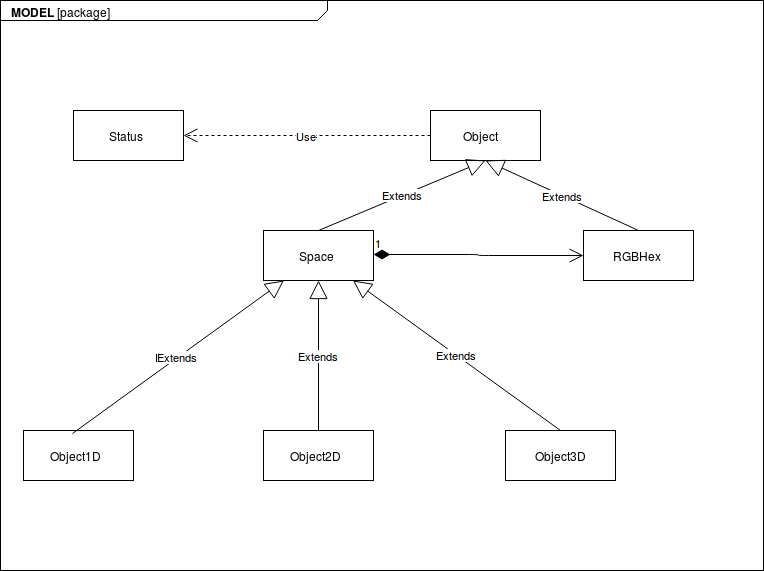
\includegraphics[scale=0.30]{Gerarchia.png}
   \caption{Gerarchia della parte Logica}
\end{figure}


\end{frame}

%------------------------------------------------

\begin{frame}
\frametitle{Classi Model}
\begin{itemize}
\item \textbf{Object} rappresenta una classe da cui deriva tutta la gerarchia, cosichè quando la \textit{BusinessLogic} andrà a fare operazioni sugli Object inseriti, a run time, eseguirà le operazioni esatte ed a aggiornerà lo \textit{Status} in modo adatto in base al tipo dinamico dell'Object selezionato.
\item \textbf{Space} classe Astratta rappresentante un Oggetto dimensionale avente un colore e una definizione di stampa (dpi), da cui poi ereditano \textit{Object1D}, \textit{Object2D} e \textit{Object3D}.
\item \textbf{Object1D} classe concreta che estende Space, possiede una lunghezza che determina se lo spazio dimensionale corrisponde a un punto unidimensionale (length=1) oppure un segmento.
\item \textbf{Object2D} classe concreta che estende Space, possiede una lunghezza e una altezza e rappresenta un sottoinsieme del piano cartesiano (oggetto bidimensionale).
\item \textbf{Object3D} classe concreta che estende Space, possiede una lunghezza, una altezza e una profondità e rappresenta un ogetto tridimensionale. 



\end{itemize}

\end{frame}

%------------------------------------------------

\begin{frame}
\frametitle{Classi Model}
\begin{itemize}
\item \textbf{RGBHex} classe concreta che deriva da Object, rappresenta un Colore RGB, costruibile tramite stringa (colore essadecimale), valori interi R G B.
Questa classe copre semplicemente il ruolo di colorare \textit{Object} e potenzialmente anche di interagire tramite operazioni su soli oggetti \textit{RGBHex}.

\item \textbf{Status} è una classe che svolge il ruolo di trasportatore; la classe Status è intrinseca in ogni classe derivante da Object, in quanto essa va ridefinita in base ai campi dati di quella classe. 

\item \textbf{BusinessLogic} è la classe che racchiude tutta la logica, tramite la funzione esegui che verrà richiamata dalla GUI con l'operatore "=" a run-time verrà scelto l'operazione adeguata ai tipi, inoltre fa da tramite con la GUI per tutto ciò che concerne la parte di Model.
\item \textbf{Exceptions} è la classe che contiene le classi di eccezioni che possono essere sollevate.
\end{itemize}
\end{frame}

%------------------------------------------------
\section{GUI}
%------------------------------------------------

\begin{frame}
\frametitle{GUI}
\begin{table}
\begin{tabular}{l l l}
\toprule
\textbf{Treatments} & \textbf{Response 1} & \textbf{Response 2}\\
\midrule
Treatment 1 & 0.0003262 & 0.562 \\
Treatment 2 & 0.0015681 & 0.910 \\
Treatment 3 & 0.0009271 & 0.296 \\
\bottomrule
\end{tabular}
\caption{Table caption}
\end{table}
\end{frame}

%------------------------------------------------

\begin{frame}
\frametitle{Theorem}
\begin{theorem}[Mass--energy equivalence]
$E = mc^2$
\end{theorem}
\end{frame}

%------------------------------------------------

\begin{frame}[fragile] % Need to use the fragile option when verbatim is used in the slide
\frametitle{Verbatim}
\begin{example}[Theorem Slide Code]
\begin{verbatim}
\begin{frame}
\frametitle{Theorem}
\begin{theorem}[Mass--energy equivalence]
$E = mc^2$
\end{theorem}
\end{frame}\end{verbatim}
\end{example}
\end{frame}

%------------------------------------------------

\begin{frame}
\frametitle{Figure}
Uncomment the code on this slide to include your own image from the same directory as the template .TeX file.
%\begin{figure}
%\includegraphics[width=0.8\linewidth]{test}
%\end{figure}
\end{frame}

%------------------------------------------------

\begin{frame}[fragile] % Need to use the fragile option when verbatim is used in the slide
\frametitle{Citation}
An example of the \verb|\cite| command to cite within the presentation:\\~

This statement requires citation \cite{p1}.
\end{frame}

%------------------------------------------------
\section{Design Pattern}
\begin{frame}
\frametitle{Design Pattern}
Strategy (do là possibilità di implementare con altri tipi di algoritmi i colori, facendo in modo che l'unica cosa disponibile a tutti sia l'interfaccia)

\end{frame}

%---------------------------------------------------

\begin{frame}
\frametitle{References}
\footnotesize{
\begin{thebibliography}{99} % Beamer does not support BibTeX so references must be inserted manually as below
\bibitem[Smith, 2012]{p1} John Smith (2012)
\newblock Title of the publication
\newblock \emph{Journal Name} 12(3), 45 -- 678.
\end{thebibliography}
}
\end{frame}

%------------------------------------------------

\begin{frame}
\Huge{\centerline{The End}}
\end{frame}

%----------------------------------------------------------------------------------------

\end{document} 
